%============================= BACKGROUND =================================

% Often used notations
\def\x{\mathbf{x}} % input vector
\def\X{\mathbf{X}} % input dataset
\def\y{\mathbf{y}} % target/output vector
\def\Y{\mathbf{Y}} % target/output dataset
\def\w{\mathbf{w}} % weight vector
\def\W{\mathbf{W}} % weight matrix
\def\b{\mathbf{b}} % bias vector
\def\h{\mathbf{h}} % hidden state
\def\R{\mathbb{R}} % real numbers
\def\L{\mathcal{L}} % loss function
\def\a{\varphi} % activation function

\def\({\left (} % left par
\def\){\right )} % right par


\chapter{Background}
\label{ch:background}

In this chapter, we present the basic concepts about \gls{dl} and an overview of the research fields on which its application has been investigated in this thesis, namely Image Classification and \gls{cbir}.
The chapter is organized as follows.
In \ref{sec:back:deep-learning}, we provide the reader with a quick introduction to \gls{dl}, focusing on deep neural networks for image and text processing and gradient-based optimization.
In \ref{sec:back:image-classification}, an introduction to image classification using convolutional neural networks is presented together with a review of successful approaches in this field.
In \ref{sec:back:image-retrieval}, we describe the main aspects of \gls{cbir} based on image representations extracted from deep neural networks, and we discuss some state-of-the-art methodologies to build effecive description of images and to efficiently index them in large-scale scenarios.
\ref{sec:back:datasets} summarizes the public datasets used in the experiments presented in this thesis.


\section{Deep Learning}
\label{sec:back:deep-learning}

\acrfull{dl} defines the set of \gls{ml} methods aiming to learn from data a \emph{hierarchy of representations} specialized for the task under consideration~\cite{goodfellow2016deep}.
\gls{dl} models are usually organized as a sequence (or more generally a graph) of parametric non-linear transformations, known as \emph{layers}, that acts like features extractors;
starting from raw data, each layer searches for useful patterns in its input and provides higher-level representation of the data to the next layer.
More formally, given an input $\x$ and $L$ non-linear transformations $f_l\(\cdot; \theta_l\)$ parametrized by $\theta_l$ ($l=1,\, \dots\,, L$), we can express the output $\y$ of the cascade of transformations as:

\begin{align} \label{eq:back:deepnet}
    \y & = f\(\x, \Theta\) \\
       & = f_L\(\dots f_2\(f_1\(\x; \theta_1\); \theta_2\); \theta_L\)
\end{align}

where $\Theta = \{\theta_l, l = 1, \dots L\}$ indicates the set of all parameters, also known as \emph{weights}.

Given a training set $\X = \{\(\x_i, \y^\star_i\), i=1,\dots,N\}$ comprised by $N$ couples of inputs and desired outputs, the quality of a particular setting of parameters is quantitatively defined by a \emph{loss function} $\L\(\X; \Theta\)$ that measures how much predictions and targets differ;
the loss function is usually defined as the average of the individual loss values computed on each sample of the dataset:

\begin{align}
    \L\(\X; \Theta\) &= \frac{1}{N} \sum_{i=1}^N \mathcal{L}\(\y_i, \y^\star_i\) \\
                   &= \frac{1}{N} \sum_{i=1}^N \mathcal{L}\(f\(\x_i; \Theta\), \y^\star_i\)
\end{align}

where the particular formulation of $\L\(\y_i, \y^\star_i\)$ is task-dependent and further discussed in \ref{subsec:back:loss}.
%In the learning phase, the model is optimized by changing the parameters $\Theta$ in such a way that the output $\mathbf{y}$ reflects the desired target $\mathbf{y^\star}$.
The learning problem is an optimization problem in which we search the best parameter setting $\Theta^\star$ that minimizes the loss function $\L\(\X; \Theta\)$:

\begin{equation} \label{eq:back:optim}
    \Theta^\star = \argmin_\Theta \L\(\X; \Theta\)
\end{equation}

% TODO add reference to similarities to mammalian brain (perceptron?)
For historical reasons, \gls{dl} models are also referred to as \emph{\glspl{dnn}} due to the resemblance of layers and their organization to the way neurons are interconnected and organized in the mammalian brain~\cite{}.
\Glspl{dnn} can be roughly categorized in \glspl{ffnn}, in which information flows from input to output in a non-recursive cascade of computations, and \glspl{rnn}, which present a feedback loop in their computation graph.
In the following sections, we will review some practical and successful formulations of \glspl{dnn},
%that are useful when dealing with image data
and we will provide the reader with the basics of gradient-based optimization of~\eqref{eq:back:optim}.

\subsection{Feed-Forward Neural Network}
\label{subsec:back:ffnn}

\Acrlongpl{ffnn} are \gls{dl} models whose computation graph can be expressed as a directed acyclic graph, i.e.\,there are no feedback loops and information flows from inputs to outputs in a cascade fashion.
Thus, when computing of the whole chain from inputs to outputs, called the \emph{forward} pass of the network, each transformation defined by layers is computed only once.

% In the following, we summarize some of the most relevant layers used in \glspl{dnn}.

%\subsubsection{Fully Connected Layer}
\subsubsection{Multilayer Perceptron}

\begin{figure}
    % TODO add figure of activations
    \caption{Commonly used activation functions in \glspl{dnn}.}
    \label{fig:back:activations}
\end{figure}

The \gls{mlp} is the simplest form of artificial neural network in the \Acrlong{dl} field.
A \gls{mlp} is comprised by a cascade of \emph{inner product} (or \emph{fully connected}) layers, which are the basic building block for \glspl{dnn}.
A inner product layer performs a linear projection of the input followed by a usually non-linear element-wise activation function.
Formally, given an input comprised by $n$ features $\x \in \R^n$, the output  $\y \in \R^m$ of the layer is obtained as follows:

\begin{equation} \label{eq:back:fully-connected}
    \y = \a \( \W \x + \b \)
\end{equation}

where $\W \in \R^{n \times m}$ and $\b \in \R^m$ are learnable parameters of a linear projection to a $m$-dimensional space.
Commonly used activation functions $\a: \R \to \R$ are the \gls{relu}, the sigmoid $\sigma\(\cdot\)$, or $\tanh\(\cdot\)$ functions (see~\Cref{fig:back:activations}).
The dimensionality of the input $n$ and of the output $m$ are referred to as respectively the number of \emph{input features} and \emph{output features}.

\begin{figure}
    \centering
    % TODO add neuron figure?
    \caption{Parallelism between real and artificial neurons in \glspl{mlp}}
    \label{fig:back:neuron}
\end{figure}

Historically, this layer implemented a group of $m$ \emph{perceptrons}.
The perceptron~\cite{rosenblatt1958perceptron} is a biologically-inspired building block for artificial neural networks that has been developed mimicking the structure of biological neurons (see \ref{fig:back:neuron}).
As a neuron cell, it is composed by $n$ inputs $\x_i$ ($i=1 \dots n$), usually connected to the output of other neurons, and a single output $\mathbf{y}$ (axon).
Each input connection is associated with a weight $\w_i$ ($i=1 \dots n$) expressing how much of the signal coming through that connection is promoted or inhibited.
Weights in a perceptron are interpreted as the strength of the interconnection between neuron cells.
The neuron ``fires'' when the combination of their weighted inputs gets above a certain threshold -- this is modelled in the perceptron defining its output as the activation function $\a$ applied to the inner product between input and weights:

\begin{equation}
    \y_j = \a \( \sum_{i=1}^n \w_i \x_i + b\)
\end{equation}

where $\y_j$ is the output of a particular neuron and $b \in \R$ is an optional weight used as bias term.
% The weight vector $\w$ is tuned in the training phase in order to
A layer composed by $m$ perceptrons (and thus $m$ outputs $\y_j, j=1 \dots m$) sharing the same input $\x$ can be formalized with ~\ref{eq:back:fully-connected}, where the columns of $\W$ correspond to the weights of the $m$ perceptrons.
% Feed-forward artificial neural networks built stacking layers of perceptrons are called \glspl{mlp}.
In \glspl{mlp}, the outputs of a layer are densely connected to the input of each neuron comprising the next layer, hence the name ``fully-connected layer''.
A \gls{mlp} with $L$ layers can be defined as follows:

\begin{equation}
    \y = \a \( \W_L \( \dots \a \( \W_2 \( \a \( \W_1 \x + \b_1 \) \) + \b_2 \) \) + \b_L \)
\end{equation}

% TODO brutto finire con la formula

\subsubsection{Convolutional Neural Network}

\begin{figure}
    \centering
    \asyinclude[inline,width=0.5\linewidth]{figures/cross-correlation2d.asy}
    \caption{Example of cross-correlation between 2D signals}
    \label{fig:back:2d-cross-corr}
\end{figure}

A \gls{cnn} is a feed-forward artificial neural network composed by at least one \emph{convolutional} layer.
This kind of layer computes the cross-correlation between the input and a set of learnable filters.
Since there is a strong similarity between the convolution and the cross-correlation operations, this layer is often attributed with the adjective ``convolutional'' in the \gls{dl} literature;
thus we will adopt the same terminology throughout this thesis.

% TODO 'local'?
The \emph{cross-correlation} (also called \emph{sliding inner product}) is typically used in signal processing to search for local matches between two signals.
Intuitively, a small signal called \emph{filter} containing the prototype we want to match is slided on a bigger input signal, and for each position, the inner product between the intersection of the two signals measures the quality of the match.
We will provide the reader with the formulation of the two-dimensional version of the cross-correlation due to its massive adoption in image-related fields that are of interest for this work.
Given a two-dimensional input matrix $\x \in \R^{H \times W}$ and a two-dimensional filter $\w \in \R^{K_1 \times K_2}$, %with $K \ll \min(H,W)$,
the cross-correlation $\y \in \R^{H' \times W'}$ between $\x$ and $\w$ expressed as follows:

\begin{equation}\label{eq:back:cross-correlation}
    \y_{u,v} = \sum_{i=1}^{K_1} \sum_{j=1}^{K_2} \w_{i,j} \x_{i+u-1,j+v-1}
\end{equation}

where $u = 1, \dots, H'$ and $v = 1, \dots W'$.
Intuitively, the filter $\w$ is superimposed on the input $\x$, and for each possible position $(u,v)$ the scalar product between the covered input and the filter is computed.
Depending on the presence of padding $P$ added to each side of the input and the stride $S$ of the filter application, the output dimensionality changes following this relations:
\begin{align*}
    H' = \left \lfloor \frac{H + 2 \times P - K_1}{S} \right \rfloor + 1 \qquad
    W' &= \left \lfloor \frac{W + 2 \times P - K_2}{S} \right \rfloor + 1
\end{align*}

Inputs and outputs of convolutional layers are also called \emph{feature maps}, since high values in the two-dimensional map is usually interpreted as the presence of a feature a particular filter has learnt to identify.
A depiction of 2D cross-correlation is reported in~\ref{fig:back:2d-cross-corr}.

\begin{figure}
    \centering
    \asyinclude[inline,width=\linewidth]{figures/convolution.asy}
    \caption{Depiction of 2D cross-correlation on volumes implemented in convolutional layers}
    \label{fig:back:convolution}
\end{figure}

\ref{eq:back:cross-correlation} defines the cross-correlation operation for inputs and outputs having both a single feature map.
Images instead are represented as 3-D tensors having $C$ channels (e.g. $C=3$ for RGB data, $C=1$ for grayscale) and two spatial dimensions $H$ and $W$;
thus, the definition of the 2D cross-correlation is extended to 3D tensors letting the filters span the depth of the input tensor.
In such way, filters are still applied over the two spatial dimensions $H$ and $W$, but each output value depends on all the input feature maps in a particular spatial position.
Formally, given an input tensor $\x \in \R^{H \times W \times C}$ and a filter $\w \in \R^{K_1 \times K_2 \times C}$ the cross-correlation $\y \in \R^{H' \times W'}$ between $\x$ and $\w$ is defined as:

\begin{equation}\label{eq:back:channel-cross-correlation}
    \y_{u,v} = \sum_{i=1}^{K_1} \sum_{j=1}^{K_2} \sum_{k=1}^C \w_{i,j,k} \x_{i+u-1,j+v-1,k}
\end{equation}

A convolution layer is often composed by a bank of $K$ filters.
Each filter is applied to the input, obtaining $K$ output feature maps that are stacked along the depth dimension.
The obtained output is a new 3D tensor $\y \in \R^{H' \times W' \times K}$ that is commonly followed by an element-wise non-linear activation $\a$.
The entire process is depicted in \ref{fig:back:convolution}.

The main difference between fully-connected layers and convolutional layers is the way weights are utilized;
while fully-connected layers have a dedicated weight for each couple of input and output features, a convolutional layer shares the weights of its filters across the spatial dimensions, thus learning to detect translation-invariant features by design.

% TODO add some cites of successful CNNs in DL literature
Convolutional layers are stacked to build deep \glspl{cnn}, that are the one of the core tools of Deep Learning for image perception and analysis \cite{}.
Once trained, filters in a deep \gls{cnn} tend to organize in a hierarchy of detectors, where layers near the input detect the presence of simple features in the input data, while the following layers build up from them and detect more complex features.
A successful example of the representative power of \glspl{cnn} is object recognition.
% TODO add a cite to object decomposition
The visual aspect of object is images follow a hierarchical organization: an object can be decomposed in parts, parts in patches, patches in textures, texture in edges or blobs, and finally in pixels \cite{}.
\begin{figure}
    % TODO is feat hier figure valuable?
    \centering
    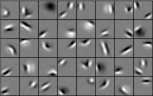
\includegraphics[height=2.9cm]{img/feat-hier-1.png}%
    \hfill%
    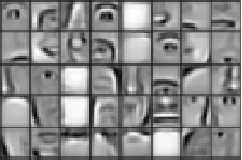
\includegraphics[height=2.9cm]{img/feat-hier-2.png}%
    \hfill%
    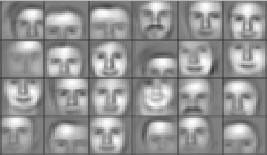
\includegraphics[height=2.9cm]{img/feat-hier-3.png}%
    \newline
    \caption{
    Visualization of the feature hierarchy learned by convolutional layers in a \gls{dl}-model trained on faces.
    Low-level features (edges and blobs, on the left) are detected and then combined to recognize parts (eyes, nose, mouth, in the middle) and finally faces (on the right).
    \figfrom{lee2011unsupervised}
    }
    \label{fig:back:filter-hier}
\end{figure}
\Glspl{cnn} trained to recognize objects, directly or indirectly, often organize their hierarchy of detectors following this kind of visual decomposition of objects (see \ref{fig:back:filter-hier}).


\subsection{Recurrent Neural Network}
\label{subsec:back:rnn}

A \acrfull{rnn} is a stateful artificial neural network in which the output depends not only on the input, but also on the current state of the network.
The state of the network acts as a memory which is updated at each input, allowing information to persist between inputs.
This architecture is naturally able to process sequences of inputs -- elements of the sequence can be fed to the network one by one, updating the internal state of the network to compactly represent the sequence processed so far regardless of its length.
% This is achieved by adding a cycle in the computation graph --

\begin{figure}
    % TODO add rnn figure (definition + unrolled)
    \centering
    \caption{Example of vanilla \acrlong{rnn}}
    \label{fig:back:rnn}
\end{figure}

Given $\x_t \in \R^n, t = 1 \dots T$ a sequence of inputs of length $T$, and $\h_t \in \R^m, t = 1 \dots T$ the hidden state of the network when all inputs until $\x_t$ have been processed, a \gls{rnn} can be described as follows:

\begin{equation}
    \h_t = f(\x_t, \h_{t-1})
\end{equation}

where $f(\cdot)$ is called the \emph{recurrent cell} of the \gls{rnn}.
In its simplest form, the recurrent cell can be implemented using a fully-connected layer that operates
on the concatenation of the current state and input:

\begin{equation}
    \h_t = \W [ \x_t || \h_{t-1} ] + \b
\end{equation}

where \W and \b are the parameters of a fully-connected layer, and $||$ is the concatenation operation.

Depending on the task we want to model, we could be interested in the last hidden state $h_T$ compactly represent the whole sequence, or we could use a combination of each hidden state $h_i$ to get access to the evolution of the information processed through time.

During learning, the \gls{rnn} is unrolled in time to the length of the input sequence to create an acyclic computation graph similar to \glspl{ffnn} on which the standard training procedures can be applied (that will be discussed in \ref{subsec:back:optim}).

\subsubsection{Long-Short Term Memory}
%LSTMs (Bidir)

\subsection{Loss Functions}
\label{subsec:back:loss}
%Loss Functions
%Cross-entropy
%MSE
%L2 Weight decay

\subsection{Gradient-Based Optimization}
\label{subsec:back:optim}
% TODO backprop (delta-rule) \cite{rumelhart1985learning}

%Backprop
%Optimizers: SGD (with momentum) / Adam
%Dropout (here?)

\section{Image Classification}
\label{sec:back:image-classification}

%Problem Setting
%Single-label binary- and multi-class image classification problem
%Examples (simple classif., sentiment analysis, etc.)
%Evaluation Metrics
%Top-k Accuracy
%AUC of ROC (TPR, FPR, confusion matrix)
%Recent Advances
%ILSVRC winners (Hybrid, VGG, Inception, Residual, ResNeXT, SENets?)
%Transfer Learning

%% probably move in the chapter
%Adversarial Examples for DNNs
%Definition
%Adv example formal definition
%Properties
%Adv. Generation Algorithms
%L-BFGS
%FGSM
%etc.
%Defense Strategies
%Change the net: Adversarial Training / other..
%Detect attacks: some rel. works on that


\section{Image Retrieval}
\label{sec:back:image-retrieval}

%Problem Setting
%CBIR (query-by-example)
%kNN schemes
%Image Representations
%Deep Features (fc7 -> RMAC)
%Permutation-based representations
%Deep Permutations
%Cross-media Retrieval
%Textual / visual / common space retrievals
%Datasets & Evaluation Metrics
%mAP, R@K, nDCG, medR, MRR

\section{Datasets}
\label{sec:back:datasets}
%ILSVRC (+Places)?, (PKLot, CNRPark)? TwitTestDataset? T4SA?
%Holidays, Oxford, Paris + distr, COCO
